Bárbara construye una cabaña de madera. La cabaña mide 42 metros de ancho.
Bárbara obtuvo varias vigas de madera de 27 metros de largo para el techo de la cabaña.
Naturalmente, quiere poner las vigas a un ángulo tal que cada par de vigas opuestas se
encuentren exactamente en el medio, como se muestra en la figura \ref{fig:techo2}:
\begin{figure}[H]
    \begin{center}
        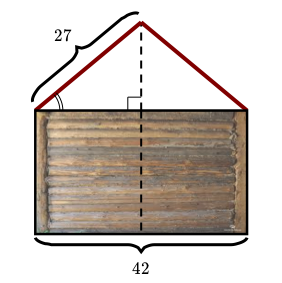
\includegraphics[width=0.25\textwidth]{../images/techo2.png}
    \end{center}
    \caption{Diagrama de la remodelación en el techo de Bob.}
    \label{fig:techo2}
\end{figure}
\textbf{¿Cuál es el ángulo de elevación de las vigas del techo en grados?}\\
\textit{Redondea tu respuesta final a la décima más cercana.}